\documentclass[a4paper,english,12pt]{article}
\usepackage{%
	amsfonts,%
	amsmath,%	
	amssymb,%
	amsthm,%
	algorithm,%
	babel,%
	bbm,%
	etex,%
	%biblatex,%
	caption,%
	centernot,%
	color,%
	dsfont,%
	enumerate,%
	epsfig,%
	epstopdf,%
	geometry,%
	graphicx,%
	hyperref,%
	latexsym,%
	mathtools,%
	multicol,%
	pgf,%
	pgfplots,%
	pgfplotstable,%
	pgfpages,%
	proof,%
	psfrag,%
	subfigure,%	
	tikz,%
	ulem,%
	url%
}	
\usepackage[noend]{algpseudocode}
\usepackage[mathscr]{eucal}
\usepgflibrary{shapes}
\usetikzlibrary{%
  	arrows,%
	backgrounds,%
	chains,%
	decorations.pathmorphing,% /pgf/decoration/random steps | erste Graphik
	decorations.text,%
	matrix,%
  	positioning,% wg. " of "
  	fit,%
	patterns,%
  	petri,%
	plotmarks,%
  	scopes,%
	shadows,%
  	shapes.misc,% wg. rounded rectangle
  	shapes.arrows,%
	shapes.callouts,%
  	shapes%
}

\theoremstyle{plain}
\newtheorem{thm}{Theorem}[section]
\newtheorem{lem}[thm]{Lemma}
\newtheorem{prop}[thm]{Proposition}
\newtheorem{cor}[thm]{Corollary}

\theoremstyle{definition}
\newtheorem{defn}[thm]{Definition}
\newtheorem{conj}[thm]{Conjecture}
\newtheorem{exmp}[thm]{Example}
\newtheorem{assum}[thm]{Assumptions}
\newtheorem{axiom}[thm]{Axiom}

\theoremstyle{remark}
\newtheorem{rem}{Remark}
\newtheorem{note}{Note}
\newtheorem{fact}{Fact}

\newcommand{\norm}[1]{\left\lVert#1\right\rVert}
\newcommand{\indep}{\!\perp\!\!\!\perp}
\DeclarePairedDelimiter\abs{\lvert}{\rvert}%
\newcommand\numberthis{\addtocounter{equation}{1}\tag{\theequation}}
\newcommand{\tr}{\operatorname{tr}}
\newcommand{\R}{\mathbb{R}}
\newcommand{\N}{\mathbb{N}}
\newcommand{\E}{\mathbb{E}}
\newcommand{\Z}{\mathbb{Z}}
\newcommand{\B}{\mathscr{B}}
\newcommand{\C}{\mathcal{C}}
\newcommand{\T}{\mathscr{T}}
\newcommand{\F}{\mathcal{F}}
\newcommand{\G}{\mathcal{G}}
%\newcommand{\ba}{\begin{align*}}
%\newcommand{\ea}{\end{align*}}
\DeclareMathOperator*{\argmax}{arg\,max}
\renewcommand{\qedsymbol}{$\blacksquare$}
\makeatletter
\def\BState{\State\hskip-\ALG@thistlm}
\makeatother

\makeatletter
\def\th@plain{%
  \thm@notefont{}% same as heading font
  \itshape % body font
}
\def\th@definition{%
  \thm@notefont{}% same as heading font
  \normalfont % body font
}
\makeatother
\date{}
%\usepackage{amsfonts}
%\usepackage{graphicx}
%\usepackage[top=1.2in,bottom=1.2in,left=1in,right=1in]{geometry}
\title{Lecture-5 }
\begin{document}
\maketitle
\begin{exmp}{Neyman-Pearson Hypothesis Testing for binary channel (contd. from previous lecture)}
\begin{figure}
\centering
\begin{tikzpicture}[scale=4]				
\draw (-0.05,0) node {${\bf 1}$} (0,0) -- (1,0) (1.05,0) node {${\bf 1}$}
node [below,midway,sloped] (TextNode) {$1-\lambda_1$};
\draw (-0.05,0.5) node {${\bf 0}$} (0,0.5) -- (1,0.5) (1.05,0.5) node {${\bf 0}$} node [above,midway,sloped] (TextNode) {$1-\lambda_0$};    
\draw (0,0) -- (1,0.5) node [pos=0.8,below] (TextNode) {$\lambda_1$} ;    
\draw (0,0.5) -- (1,0) node [pos=0.8,above] (TextNode) {$\lambda_0$} ;    
\end{tikzpicture}
\caption{The Binary Channel}
\end{figure}
Likelihood ratio is given by  $ L(y) = \frac{{P}_1(y)}{{P}_0(y)} $. Decision rule for Neyman Pearson testing is given by,
\begin{equation}
\tilde{\delta}_{NP} (y)=
\begin{cases}
1,\hspace{10pt}L(y) > \eta_0,\\ 
\gamma_0,\hspace{5pt}L(y)= \eta_0,\\
0,\hspace{10pt}L(y) < \eta_0,\\
\end{cases}
\end{equation}
where $\eta_0$ is desired threshold for $\alpha$ level Neyman Pearson testing.
\begin{equation}
%L(0) = \frac{\mathbb{P}_1(0)}{\mathbb{P}_0(0)} = \frac{\lambda_1}{1-\lambda_0} ; \\
%L(1) = \frac{\mathbb{P}_1(1)}{\mathbb{P}_0(1)} = \frac{1-\lambda_1}{\lambda_0};\\
L(y) = \begin{cases}
\frac{\lambda_1}{1-\lambda_0},\hspace{5pt}y=0,  \\ 
\frac{1-\lambda_1}{\lambda_0},\hspace{5pt}y=1.
\end{cases}
\end{equation}
Assuming $\lambda_0 + \lambda_1 < 1$, we get,
\begin{eqnarray}
1-\lambda_0 > \lambda_1,\hspace{5pt}\mbox{or}\hspace{5pt}1-\lambda_1 > \lambda_0.
\end{eqnarray}
Now $\frac{\lambda_1}{1-\lambda_0} = \frac{\lambda_1}{>\lambda_1}$
\{from equation (1)\} 
$\frac{1-\lambda_1}{\lambda_0} = \frac{>\lambda_0}{\lambda_0}$
\{from equation (2)\} 
\begin{eqnarray}
&\Rightarrow \frac{\lambda_1}{1-\lambda_0} < 1& \\
&\Rightarrow \frac{1-\lambda_1}{\lambda_0} > 1&
\end{eqnarray}
use equations (3) and (4) 
\begin{equation}
\frac{\lambda_1}{1-\lambda_0} < \frac{1-\lambda_1}{\lambda_0}
\end{equation}
\begin{equation}
\mathbb{P}_0 (L(y) > \eta)=\begin{cases}
1\hspace{10pt}\mbox{if}\hspace{3pt}\eta< \frac{\lambda_1}{1-\lambda_0},\\ 
\lambda_0\hspace{5pt}\mbox{if}\hspace{3pt}\frac{\lambda_1}{1-\lambda_0} \leq \eta \geq \frac{1-\lambda_1}{\lambda_0},\\
0\hspace{10pt}\mbox{if}\hspace{3pt}\eta \geq  \frac{1-\lambda_1}{\lambda_0}.
\end{cases}
\end{equation}
\begin{figure}[t]
\centering
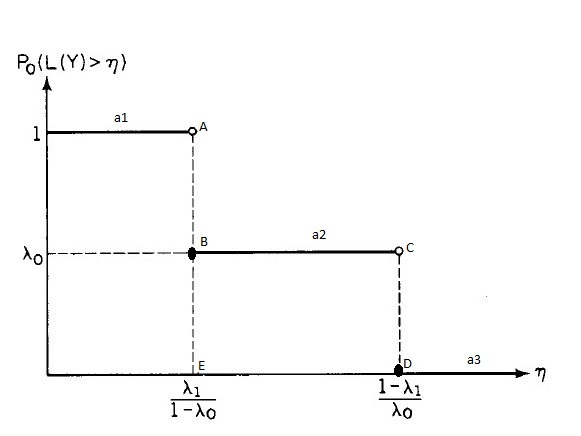
\includegraphics[scale=0.8]{Figures/img.jpg} 
\caption{Curve for threshold and randomization selection for a binary channel}
\end{figure}
Let $\eta_0$ be the smallest number such that,
\begin{equation}
\mathbb{P}_0(p_1(Y) > \eta_0 p_0(Y)) \leq \alpha.
\end{equation}
\begin{equation}
\eta_0 =\begin{cases}
\frac{1-\lambda_1}{\lambda_0},\hspace{10pt}\alpha \in [0,\lambda_0),~~\mbox{(section $a_3$)}\\
\frac{\lambda_1}{1-\lambda_0},\hspace{10pt}\alpha \in [\lambda_0,1),~~\mbox{(section $a_2$)}\\
\mbox{arbitrary},\hspace{10pt}\alpha = 1.
\end{cases}
\end{equation}
If $\mathbb{P}_0(p_1(Y) > \eta_0 p_0(Y)) <\alpha$, choose  
\begin{equation}
\gamma_0 = \frac{\alpha-\mathbb{P}_0(p_1(Y) > \eta_0 p_0(Y))}{\mathbb{P}_0(p_1(Y) = \eta_0 p_0(Y))}
\end{equation}
If $\alpha \in [0,\lambda_0)$,
\begin{equation}
\gamma_0 = \frac{\alpha-0}{\mathbb{P}_0(p_1(Y) = \eta_0 p_0(Y))}
\end{equation}
and,
\begin{equation}
\mathbb{P}_0(p_1(Y) = \eta_0 p_0(Y)) = \lambda_0-0
\end{equation}
which is equal to the jumpsize at threshold, CD in fig-2.
\begin{equation}
\gamma_0 = \frac{\alpha}{\lambda_0}
\end{equation}
If $\alpha \in [\lambda_0,1)$,
\begin{equation}
\mathbb{P}_0(p_1(Y) = \eta_0 p_0(Y)) = 1-\lambda_0
\end{equation}
which is the jumpsize at threshold, AB in fig-2. We get, $\gamma_0 = \frac{\alpha-\lambda_0}{1-\lambda_0}$.
\begin{equation}
\gamma_0=\begin{cases}
\frac{\alpha}{\lambda_0},\hspace{45pt}\alpha \in [0,\lambda_0),\\
\frac{\alpha-\lambda_0}{1-\lambda_0},\hspace{32pt}\alpha \in [\lambda_0,1),\\
\mbox{arbitrary},\hspace{10pt}\alpha = 1.
\end{cases}
\end{equation}
If $\alpha \in [0,\lambda_0)$, 
\begin{equation}
\tilde{\delta}_{NP} (y) =\begin{cases}
\frac{\alpha}{\lambda_0},\hspace{10pt}\mbox{if}~y=1,\\
0,\hspace{15pt}\mbox{if}~y=0.\\
\end{cases}
\end{equation}
If $\alpha \in [\lambda_0,1]$,
\begin{equation}
\tilde{\delta}_{NP} (y) =\begin{cases}
1,\hspace{32pt}\mbox{if}~y=1,\\
\frac{\alpha - \lambda_0}{1-\lambda_0},\hspace{15pt}\mbox{if}~y=0.\\
\end{cases}
\end{equation}
The detection probability of the Neyman-Pearson test is given by 
\begin{eqnarray}
\mathbb{P}_D (\tilde{\delta}_{NP}) =\mathbb{P}_1(L(Y) > \eta_0) + \gamma_0 \mathbb{P}_1(L(Y) = \eta_0),\\\nonumber
\mathbb{P}_D (\tilde{\delta}_{NP}) =\begin{cases}
\frac{\alpha (1-\lambda_1)}{\lambda_0},\hspace{80pt}\alpha \in [0,\lambda_0),\\
(1-\lambda_1) + \frac{\lambda_1 (\alpha -\lambda_0)}{1-\lambda_0},\hspace{20pt}\alpha \in [\lambda_0,1].
\end{cases}
\end{eqnarray}
\end{exmp}
\section{Composite Hypothesis Test}
The hypothesis testing problems discussed in the previous lectures are sometimes known as simple hypothesis testing problems because each of the two hypotheses corresponds to only a single distribution for the observation. In many hypothesis testing problems, however, there are many possible distributions that can occur under each of the hypotheses. Hypotheses of this type are known as \textit{Composite Hypotheses}.
\par To model the most general type of composite-hypotheses testing problem, we can consider a family of probability distributions on $\Gamma$ indexed by a parameter $\theta$ taking values in a parameter set $\Lambda$. That is, we have a family,
\begin{equation}
\{P_\theta;\theta \in \Lambda\}
\end{equation}
$\Lambda$=\{set of all possible states of nature\}.
\begin{exmp}
For the simple hypothesis test $\Lambda$ =\{0,1\}. More generally,we might have a parameter space that is the union of two disjoint parameter sets $\Lambda_0$ and $\Lambda_1$ representing the ranges of the parameter under the two hypotheses. 
\end{exmp}
\subsection*{Bayesian Formulation:}
In a Bayesian formulation of the composite hypothesis testing problem, we assume that the parameter is a random quantity, $\Theta$, taking on the values in $\Lambda$, i.e.,
\begin{equation}
\Theta : \Omega \to \Lambda 
\end{equation}
In this case $ P_\theta$ is interpreted as the conditional distribution of Y given that $\Theta = \theta$.
\begin{equation}
P_\theta \{ Y = y \} = \mathbb{P} \{ Y=y | \Theta = \theta\} 
\end{equation}
we will consider only non randomized decision rules, $ \Theta \in \Lambda_0~~or~~\Lambda_1$. To choose an optimum decision rule, assign cost to our decisions through a cost function $ C_i (\theta)$, where, $ C_i (\theta)$ is the cost of choosing decision $i \in \{0,1\}$ when $Y \sim P_\theta$. Assume that $C$ is nonnegative and bounded. For a decision rule $\delta$, the conditional risk is,
\begin{eqnarray}
R_\theta (\delta) = \mathbb{E} [ C_{ \delta_y } (\theta)]
\end{eqnarray}
where $\mathbb{E}$ denotes expectation assuming that $ Y \sim P_\theta$. Bayes risk can be defined as 
\begin{equation}
r(\delta) = \mathbb{E} [ R_\Theta (\delta)]
\end{equation}
Bayes rule defined as minimization of $r(\delta)$.
\begin{align}
r(\delta) &= \mathbb{E} [ R_\Theta (\delta)]\hspace{20pt}{using\,\, equation(6)}\\\nonumber
&= \mathbb{E}[\mathbb{E}[ C_{ \delta_y } (\Theta)]]\\\nonumber
&= \mathbb{E}[\mathbb{E}[ C_{ \delta_y } (\theta) | \Theta ]]\\\nonumber
&= \mathbb{E}[\mathbb{E}[ C_{ \delta_y } (\Theta) | Y=y ]]\hspace{10pt} \forall \{ y \in \Lambda \}.
\end{align}
Minimizing $r(\delta)$ is same as minimizing $\mathbb{E}[\mathbb{E}[ C_{ \delta_y } (\Theta) | Y=y ]$. Since $\delta_y $ can only be 0 or 1, we thus see that Bayes rule is given by, 
\begin{equation}
\delta_y = \underset{i \in \{0,1\}}{\arg\min}~\mathbb{E}[C_{ \delta_y } (\Theta) | Y=y]
\end{equation}
We choose $\delta (y)$ to be the decision that minimizes the posterior cost.
\begin{equation}
\delta_y =\mathbb{I}_{\{\mathbb{E}[C_1(\Theta) | Y=y] < \mathbb{E}[C_0(\Theta) | Y=y]\}}
\end{equation} 
$\delta (y)$ chooses the hypothesis that is least costly. For example, when $\Lambda =\{0,1\}$, $\delta (y)$ reduces with the Bayes rule for simple hypothesis test. Assume costs being uniform i.e., $ C_i (\theta) = C_{ij}~\forall\theta \in \Lambda_j $.
\begin{align}
&=\int_{\theta \in \Lambda_1} C_{11} d\mathbb{P}_{(\theta | Y=y)} +  \int_{\theta \in \Lambda_0} C_{10} d\mathbb{P}_{(\theta | Y=y)},\\\nonumber
&=C_{11} \mathbb{P}(\Theta \in \Lambda_1  | Y=y)  + C_{10}  \mathbb{P}(\Theta \in \Lambda_0  | Y=y),\\\nonumber
&< C_{01} \mathbb{P}(\Theta \in \Lambda_1  | Y=y)+C_{00}  \mathbb{P}(\Theta \in \Lambda_0  | Y=y).
\end{align}
Here we assume that $ C_{11} < C_{01}$. We can also write,
\begin{equation}
\Gamma_1 =\left\{y\in \Gamma : \frac{C_{10}-C_{00}}{C_{01}-C_{11}} < \frac{\mathbb{P}(\Theta \in \Lambda_1  | Y=y)}{\mathbb{P}(\Theta \in \Lambda_0  | Y=y)} \right\}
\end{equation}
where $\mathbb{P}(\Theta \in \Lambda_j  | Y=y)$ denotes the conditional probability that $\Theta$ lies in $\Lambda_j$ given that $Y=y$.Assume Y has conditional densities $\mathbb{P} (y | \Theta \in \Lambda_j)$ for j=0,1. Bayes formula implies that : 
\begin{equation}
\mathbb{P} ( \Theta \in \Lambda_j | Y=y) = \frac{{\mathbb{P} (Y=y | \Theta \in \Lambda_j)}{\mathbb{P}(\Theta \in \Lambda_j)}}{\mathbb{P}(y)},~j=0,1.
\end{equation}
We can write $\Gamma_1$ as 
\begin{equation}
\Gamma_1 =\left\{ \frac{{d\mathbb{P} (Y=y | \Theta \in \Lambda_1)}{\mathbb{P}(\Theta \in \Lambda_1)}}{{d\mathbb{P} (Y=y | \Theta \in \Lambda_0)}{\mathbb{P}(\Theta \in \Lambda_0)}} > \frac{C_{10}-C_{00}}{C_{01}-C_{11}}\right\}.
\end{equation}
For general case, let $\Theta \sim W,~Y\sim \mathbb{P}_\theta,~\theta \in \Lambda $,
\begin{equation}
d\mathbb{P}[Y\leq y | \Theta \in \Lambda_j] = \int_\Lambda {\mathbb{P}_\theta(y) dW_j(\theta)},
\end{equation}
where,
\begin{equation}
dW_j(\theta)\begin{cases}
0,\hspace{50pt}\theta \notin \Lambda_j,\\
\frac{dW(\theta)}{\mathbb{P}\{\theta \in \Lambda_j\}},\hspace{20pt}\theta \in \Lambda_j.
\end{cases}
\end{equation}
\end{document}